\chapter{Preliminaries}

\section{Introduction}
To be written once we know where everything is going to go.

%%%%%%%%%%%%%%%%%%%%%%%%%

\section{Coxeter Systems}\label{sec:coxeter}
A \emph{Coxeter system} is a pair $(W,S)$ consisting of a finite set $S$ of generating involutions and a group $W$, called a \emph{Coxeter group}, with presentation 
\[ 
W = \langle S \mid (st)^{m(s, t)} = e \text{ for } m(s, t) < \infty \rangle,
\]
where $e$ is the identity, $m(s,t) = 1$ if and only if $s = t$, and $m(s,t) = m(t,s)$. It turns out that the elements of $S$ are distinct as group elements and that $m(s,t)$ is the \emph\emph{order} of $st$~\cite{Humphreys1990}. We call $m(s,t)$ the \emph{bond strength} of $s$ and $t$.\\

Since $s$ and $t$ are elements of order 2, the relation $(st)^{m(s,t)}=e$ can be written as
\begin{equation}\label{braid} 
	\underbrace{sts \cdots}_{m(s,t)}=\underbrace{tst\cdots}_{m(s,t)}
\end{equation}
with $m(s,t) \geq 2$ factors. If $m(s,t)=2$, then $st=ts$ is called a \emph{commutation relation} and $s$ and $t$ commute. Otherwise, if $m(s,t) \geq 3$, then the relation in \eqref{braid} is called a \emph{braid relation}. Replacing $\underbrace{sts\cdots}_{m(s,t)}$ with $\underbrace{tst\cdots}_{m(s,t)}$ will be referred to as a \emph{braid move} if $m(s,t) \geq 3$ and a \emph{commutation} if $m(s,t)=2$.\\

We can represent a Coxeter system $(W,S)$ with a unique \emph{Coxeter graph} $\Gamma$ having
\begin{enumerate}
\item vertex set $S$ and
\item edges $\{s, t\}$ for each $m(s,t) \geq 3$.	
\end{enumerate}

Each edge $\{s, t\}$ is labeled with its corresponding bond strength $m(s,t)$. Since $m(s,t)=3$ occurs most frequently, it is customary to leave the edge unlabeled. If $(W,S)$ is a Coxeter group with corresponding Coxeter system $\Gamma$, we may denote the Coxeter group as $W(\Gamma)$ and the generating set as $S(\Gamma)$ for clarity. There is a one-to-one correspondence between Coxeter systems and Coxeter graphs. That is, given a Coxeter graph $\Gamma$, we can uniquely reconstruct the corresponding Coxeter system. Note that $s$ and $t$ are not connected in the graph if and only if $m(s,t)=2$. Also, the Coxeter group $W(\Gamma)$ is said to be \emph{irreducible} if and only if $\Gamma$ is connected. Otherwise, $W(\Gamma)$ is said to be \emph{reducible}. Furthermore, if the graph is disconnected, the connected components correspond to factors in a direct product of irreducible Coxeter groups~\cite{Humphreys1990}.

\begin{example}
~
\begin{itemize}
\item[(a)~] The Coxeter graph of type $A_n$ is given in Figure~\ref{fig:A}. Given $A_n$, we can construct the corresponding Coxeter system\ with generating set $S(A_n)=\{s_1, s_2, \ldots s_n\}$ and defining relations
\begin{enumerate}
	\item $s_i^2=e$ for all $i$;
	\item $s_is_j=s_js_i$ when $|i-j|>1$;
	\item $s_is_js_i=s_js_is_j$ when $|i-j|=1.$
\end{enumerate}
The Coxeter group $W(A_n)$ is isomorphic to the symmetric group $\Sym_{n+1}$ under the correspondence $s_i \mapsto (i, i+1)$, where $(i, i+1)$ is the adjacent transposition that swaps $i$ and $i+1$.
\item[(b)~] The Coxeter graph of type $B_n$ is given in Figure~\ref{fig:B}. From $B_n$, we can construct the corresponding Coxeter system with generating set $S(B_n)=~\{s_0,s_1, \ldots s_{n-1}\}$ and defining relations
\begin{enumerate}
	\item $s_i^2=e$ for all $i$;
	\item $s_is_j=s_js_i$  when $|i-j|>1$;
	\item $s_is_js_i=s_js_is_j$ when $|i-j|=1$ for $i,j \in \{1,2,\ldots, n-1\}$;
	\item $s_0s_1s_0s_1=s_1s_0s_1s_0$.
\end{enumerate}
The Coxeter group $W(B_n)$ is isomorphic to $\Sym_n^B$, where $\Sym_n^B$ is the group of all signed permutations on the set $\{1,2, \ldots,n\}$. 
\item[(c)~] The Coxeter graph of type $\widetilde C_n$ is seen in Figure~\ref{fig:affC}. From $\widetilde C_n$, we can construct the Coxeter group $W(\widetilde C_n)$ with generating set $S(\widetilde{C}_n)=~\{s_0, s_1, \ldots s_n\}$ and defining relations 
\begin{enumerate}
	\item $s_i^2=e$ for all $i$;
	\item $s_is_j=s_js_i$ when $|i-j|>1$ for $i \in \{1,2, \ldots, n-1\}$;
	\item $s_is_js_i=s_js_is_j$ 	when $|i-j|=1$ for $i \in \{1,2, \ldots, n-1\}$;
	\item $s_0s_1s_0s_1=s_1s_0s_1s_0$;
	\item $s_ns_{n-1}s_ns_{n-1}=s_{n-1}s_ns_{n-1}s_n.$
\end{enumerate}
\end{itemize}
\end{example}

In Figures~\ref{fig:fincoxgraphs} and~\ref{fig:infincoxgraphs} all irreducible finite and some irreducible infinite Coxeter graphs are given. The Coxeter graphs in Figure~\ref{fig:fincoxgraphs} correspond to the finite Coxeter groups, while the Coxeter graphs in Figure~\ref{fig:infincoxgraphs} are the irreducible affine Coxeter groups, which are infinite. This thesis will mainly focus upon Coxeter groups of types $A_n, B_n$ and $\widetilde{C_n}$ and will also briefly touch upon types $\widetilde{A}_n$ and $F_n$.

Given a Coxeter system $(W,S)$, a word $s_{x_1}s_{x_2} \cdots s_{x_m}$ in the free monoid $S^*$ on $S$ is called an \emph{expression} for $w \in W$ if it is equal to $w$ when considered as a group element. If $m$ is minimal among all expressions for $w$, the corresponding word is called a \emph{reduced expression} for $w$. In this case, we define the \emph{length} of $w$ to be $l(w):= m$. Each element $w \in W$ may have multiple reduced expressions that represent it. If we wish to emphasize a specific, possibly reduced, expression for $w \in W$ we will represent it as $\overline{w}=s_{x_1}s_{x_2}\cdots s_{x_m}.$ The following theorem tells us more about how reduced expressions for a given group element are related.

\begin{theorem} [Matsumoto, \cite{Geck2000}]
	If $w \in W$, then given a reduced expression for $w$ we can obtain every other reduced expression for $w$ by a sequence of braid moves and commutations of the form
	\[\underbrace{sts\cdots}_{m(s,t)} \rightarrow \underbrace{tst\cdots}_{m(s,t)}\]
	where $s,t \in S$ and $m(s,t) \geq 2$. \qed
\end{theorem}
 
It follows from Matsumoto's Theorem that if a generator $s_i$ appears in a reduced expression for $w \in W$, then $s$ appears in all reduced expressions for $w$. Let $w \in W$ and fix a reduced expression $\overline{w}$ for $w$. Then the \emph{support} of $w$, denoted $\supp(w)$, is the set of all generators of that appear in $w$. It follows from Matsumoto's Theorem that $s$ appears in $\supp(\overline{w})$ if and only if $s$ appears in the support of all reduced expressions for $w$. If $\supp(w)=S$, we say that $w$ has \emph{full support}. 

Given $w \in W$ and a fixed reduced expression $\overline{w}$ for $w$, any subsequence of $\overline{w}$ is called a \emph{subexpression} of $\overline{w}$. We will refer to a subexpression consisting of consecutive subsequence of $\overline{w}$ as a \emph{subword} of $\overline{w}$.\\

\begin{example}
Let $w \in W(A_7)$ and let $\overline{w}=s_7s_2s_4s_5s_3s_2s_3s_6$ be a fixed expression for $w$. Then we have
\begin{align*}
s_7\textcolor{blue}{s_2s_4}s_5s_3s_2s_3s_6&=s_7s_4\textcolor{blue}{s_2s_5}s_3s_2s_3s_6\\
&=s_7s_4s_5\textcolor{orange}{s_2s_3s_2} s_3s_6\\
&=s_7s_4s_5s_3s_2\textcolor{red}{s_3s_3}s_6\\
&=s_7s_4s_5s_3s_2s_6,
\end{align*}
where the \textcolor{blue}{blue} highlighted text corresponds to a commutation, the \textcolor{orange}{orange} highlighted text corresponds to a braid move, and the \textcolor{red}{red} highlighted text corresponds to two elements that create the identity. This shows that $\overline{w}$ is not reduced. However it turns out that, $s_7s_4s_5s_3s_2s_6$ is reduced. Thus $l(w)=6$ and $\supp(w)=\{s_2, s_3, s_4, s_5, s_6, s_7\}$.
\end{example}

Let $(W,S)$ be a Coxeter system of type $\Gamma$ and let $w \in W(\Gamma)$. We define the \emph{left descent set} and \emph{right descent set} of $w$ as follows:
\[\mathcal{L}(w):=\{s \in S \mid l(sw) < l(w)\}\]
and
\[\mathcal{R}(w):=\{s \in S \mid l(ws) < l(w)\}.\]
In~\cite{Bjorner2005} it is shown that $s \in \mathcal{L}(w)$ (respectively, $s \in \mathcal{R}(w)$) if and only if there is a reduced expression for $w$ that begins with $s$ (respectively, there is a reduce expression for $w$ that ends with $s$).

\begin{example}
Let $w \in W(B_4)$ such that all reduced expressions for $w$ are as follows 
$$\begin{array}{ll}
s_0s_1s_2s_1s_3 & s_0s_2s_1s_2s_3\\
s_0s_1s_2s_3s_1 & s_2s_0s_1s_2s_3	
\end{array}$$
We see that $l(w)=5$ and $w$ has full support. Also, we see that $\mathcal{L}(w)=\{s_0, s_2\}$ while $\mathcal{R}(w)=\{s_1, s_3\}$.	
\end{example}

\begin{figure}[h!]
\begin{tabular}{m{7cm} m{7cm}}
\begin{subfigure}{0.5\textwidth} \centering
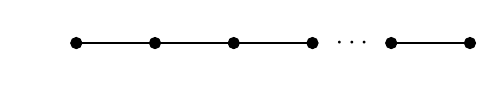
\begin{tikzpicture}[scale=1.0]%A_{n}
\draw[fill=black] \foreach \x in {1,2,...,6} {(\x,10) circle (2pt)};
\draw {(.5,10) node{}
(4.5,10) node{$\cdots$}
[-] (1,10) -- (4,10)
[-] (5,10) -- (6,10)
(1,10) node{}}; 
\end{tikzpicture}
\caption{$A_{n}$} \label{fig:A}
\end{subfigure} &

\begin{subfigure}{0.5\textwidth} \centering
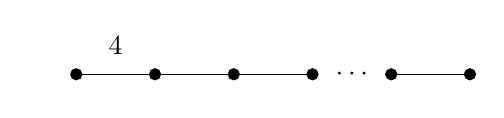
\begin{tikzpicture}[scale=1.0]%B_{n}
\draw [fill=black] \foreach \x in {1,2,...,6} {(\x,8.5) circle (2pt)};
\draw {(.5,8.5) node{}
(1.5,8.5) node[label=above:$4$]{}
(4.5,8.5) node{$\cdots$}
[-] (1,8.5) -- (4,8.5)
[-] (5,8.5) -- (6,8.5)
(2,8.5) node{}}; 
\end{tikzpicture}
\caption{$B_{n}$} \label{fig:B}
\end{subfigure} \\

    & \\ 

\begin{subfigure}{0.5\textwidth} \centering
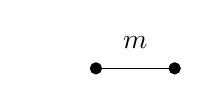
\begin{tikzpicture}[scale=1.0]
\draw[fill=black] \foreach \x in {1,2} {(\x,0) circle (2pt)};
\draw {(.25,0) node{}
(1.5,0) node[label=above:$m$]{}
[-] (1,0) -- (2,0)
(2,0) node{}};
\end{tikzpicture}
\caption{$I_{2}(m)$} \label{fig:I}
\end{subfigure} &

\begin{subfigure}{0.5\textwidth} \centering
\begin{tikzpicture}[scale=1.0]
\draw[fill=black] \foreach \x in {1,2,...,6} {(\x,6.5) circle (2pt)};%D_{n}
\draw[fill=black] (2,7.5) circle (2pt);
\draw {(.5,6.5) node{}
(4.5,6.5) node{$\cdots$}
[-] (1,6.5) -- (4,6.5)
[-] (5,6.5) -- (6,6.5)
[-] (2,6.5) -- (2,7.5)
(2,6.5) node{}};
\end{tikzpicture}
\caption{$D_{n}$} \label{fig:D}
\end{subfigure} \\

    & \\ 
    
\begin{subfigure}{0.5\textwidth} \centering
\begin{tikzpicture}[scale=1.0]%E_{6}
\draw[fill=black] \foreach \x in {1,2,...,5} {(\x,4.5) circle (2pt)};
\draw[fill=black] (3,5.5) circle (2pt);
\draw {
[-] (1,4.5) -- (5,4.5)
[-] (3,4.5) -- (3,5.5)
(3,4.5) node{}};
\end{tikzpicture}
\caption{$E_{6}$} \label{fig:E6}
\end{subfigure} &



\begin{subfigure}{0.5\textwidth} \centering
\begin{tikzpicture}[scale=1.0]%E_{7}
\draw[fill=black] \foreach \x in {1,2,...,6} {(\x,4.5) circle (2pt)};
\draw[fill=black] (3, 5.5) circle (2pt);
\draw {
[-] (1,4.5) -- (5,4.5)
[-] (5,4.5) -- (6,4.5)
[-] (3,4.5) -- (3,5.5)
(3,4.5) node{}};
\end{tikzpicture}
\caption{$E_{7}$} \label{fig:E7}
\end{subfigure} \\

    & \\ 


\begin{subfigure}{0.5\textwidth} \centering
\begin{tikzpicture}[scale=1.0]%E_{8}
\draw[fill=black] \foreach \x in {1,2,...,7} {(\x,4.5) circle (2pt)};
\draw[fill=black] (3,5.5) circle (2pt);
\draw {
[-] (1,4.5) -- (7,4.5)
[-] (3,4.5) -- (3,5.5)
(3,4.5) node{}};
\end{tikzpicture}
\caption{$E_{8}$} \label{fig:E6}
\end{subfigure} &

\begin{subfigure}{0.5\textwidth} \centering
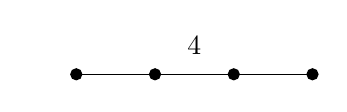
\begin{tikzpicture}[scale=1.0]%F_{4}
\draw[fill=black] \foreach \x in {1,2,...,4} {(\x,3) circle (2pt)};
\draw {(.5,3) node{}
(2.5,3) node[label=above:$4$]{}
[-] (1,3) -- (4,3)
(3,3) node{}};
\end{tikzpicture}
\caption{$F_{4}$} \label{fig:F4}
\end{subfigure} \\

&\\

\begin{subfigure}{0.5\textwidth} \centering
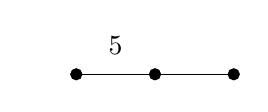
\begin{tikzpicture}[scale=1.0]
\draw[fill=black] \foreach \x in {1,2,...,3} {(\x,1.5) circle (2pt)};%H_{3}
\draw {(.5,1.5) node{}
(1.5,1.5) node[label=above:$5$]{}
[-] (1,1.5) -- (3,1.5)
(2,1.5) node{}}; 
\end{tikzpicture}
\caption{$H_{3}$} \label{fig:H}
\end{subfigure} &

\begin{subfigure}{0.5\textwidth} \centering
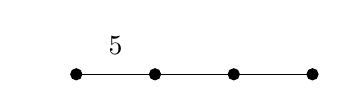
\begin{tikzpicture}[scale=1.0]
\draw[fill=black] \foreach \x in {1,2,...,4} {(\x,1.5) circle (2pt)};%H_{4}
\draw {(.5,1.5) node{}
(1.5,1.5) node[label=above:$5$]{}
[-] (1,1.5) -- (4,1.5)
(2,1.5) node{}}; 
\end{tikzpicture}
\caption{$H_{4}$} \label{fig:H}
\end{subfigure}
\end{tabular}
\caption{Coxeter graphs corresponding to the irreducible finite Coxeter groups.}
\label{fig:fincoxgraphs}
\end{figure}

%%%%%%%%%%%%%%%%%%%%%%%%%%%

\begin{figure}[h!]
\begin{tabular}{m{7cm} m{7cm}}
\begin{subfigure}{0.5\textwidth} \centering
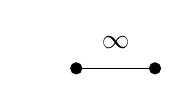
\begin{tikzpicture}[scale=1.0]%\widetilde{A}_{2}
\draw[fill=black] \foreach \x in {1,2} {(\x,10) circle (2pt)};
\draw { (.5,10) node{}
(1.5,10) node[label=above:$\infty$]{}
[-] (1,10) -- (2,10)
(1,10) node{}}; 
\end{tikzpicture}
\caption{$\widetilde{A}_{1}$} \label{fig:affA1}
\end{subfigure} &

\begin{subfigure}{0.5\textwidth} \centering
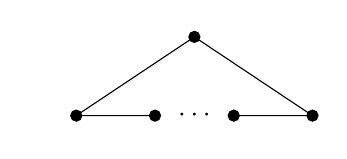
\begin{tikzpicture}[scale=1.0]%\widetilde{A}_{n}
\draw [fill=black] \foreach \x in {1,...,4} {(\x,7.5) circle (2pt)};
\draw [fill=black] (2.5, 8.5) circle (2pt);
\draw {(.5,8.5) node{}
(2.5,7.5) node{$\cdots$}
[-] (2.5,8.5) -- (1, 7.5)
[-] (2.5,8.5) -- (4, 7.5)
[-] (1,7.5) -- (2,7.5)
[-] (3,7.5) -- (4,7.5)
(2,8.5) node{}}; 
\end{tikzpicture}
\caption{$\widetilde{A}_{n}$} \label{fig:affAn}
\end{subfigure} \\

    & \\ 

\begin{subfigure}{0.5\textwidth} \centering
\begin{tikzpicture}[scale=1.0]%\widetilde{B}_{n}
\draw[fill=black] \foreach \x in {1,2,...,6} {(\x,0) circle (2pt)};
\draw[fill=black] (2,1) circle (2pt);
\draw {(.25,0) node{}
(5.5,0) node[label=above:$4$]{}
(4.5, 0) node{$\cdots$}
[-] (1,0) -- (4,0)
[-] (5,0) -- (6,0)
[-] (2,1) -- (2,0)
(2,0) node{}};
\end{tikzpicture}
\caption{$\widetilde{B}_{n}$} \label{fig:affB}
\end{subfigure} &

\begin{subfigure}{0.5\textwidth} \centering
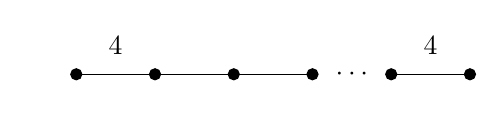
\begin{tikzpicture}[scale=1.0]
\draw[fill=black] \foreach \x in {1,2,...,6} {(\x,5) circle (2pt)};%\widetild{C}_{n}
\draw {(.5,5) node{}
(4.5,5) node{$\cdots$}
(5.5,5) node[label=above:$4$]{}
(1.5,5) node[label=above:$4$]{}
[-] (1,5) -- (4,5)
[-] (5,5) -- (6,5)
(2,5) node{}};
\end{tikzpicture}
\caption{$\widetilde{C}_{n}$} \label{fig:affC}
\end{subfigure} \\

    & \\ 
    
\begin{subfigure}{0.5\textwidth} \centering
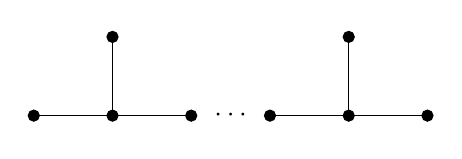
\begin{tikzpicture}[scale=1.0]%\widetilde{D}_{6}
\draw[fill=black] \foreach \x in {1,2,...,6} {(\x,3.5) circle (2pt)};
\draw[fill=black] (2,4.5) circle (2pt);
\draw[fill=black] (5,4.5) circle (2pt);
\draw {
(3.5,3.5) node{$\cdots$}
[-] (1,3.5) -- (3,3.5)
[-] (4, 3.5) --(6, 3.5)
[-] (2,3.5) -- (2,4.5)
[-] (5,3.5)-- (5,4.5)
(3,4.5) node{}};
\end{tikzpicture}
\caption{$\widetilde{D}_{n}$} \label{fig:E6}
\end{subfigure} &



\begin{subfigure}{0.5\textwidth} \centering
\begin{tikzpicture}[scale=1.0]%\widetilde{E}_{6}
\draw[fill=black] \foreach \x in {1,2,...,5} {(\x,4.5) circle (2pt)};
\draw[fill=black] (3, 5.5) circle (2pt);
\draw[fill=black] (3, 6.5) circle (2pt);
\draw {
[-] (1,4.5) -- (5,4.5)
[-] (3,4.5) -- (3,6.5)
(3,4.5) node{}};
\end{tikzpicture}
\caption{$\widetilde{E}_{6}$} \label{fig:affE6}
\end{subfigure} \\

    & \\ 


\begin{subfigure}{0.5\textwidth} \centering
\begin{tikzpicture}[scale=1.0]%\widetilde{E}_{7}
\draw[fill=black] \foreach \x in {1,2,...,7} {(\x,4.5) circle (2pt)};
\draw[fill=black] (4,5.5) circle (2pt);
\draw {
[-] (1,4.5) -- (7,4.5)
[-] (4,4.5) -- (4,5.5)
(3,4.5) node{}};
\end{tikzpicture}
\caption{$\widetilde{E}_{7}$} \label{fig:affE7}
\end{subfigure} &

\begin{subfigure}{0.5\textwidth} \centering
\begin{tikzpicture}[scale=1.0]%\widetilde{E}_{8}
\draw[fill=black] \foreach \x in {1,2,...,8} {(\x,3) circle (2pt)};
\draw[fill=black] (3,4) circle (2pt);
\draw {(.5,3) node{}
[-] (3,4) -- (3,3)
[-] (1,3) -- (8,3)
(3,3) node{}};
\end{tikzpicture}
\caption{$\widetilde{E}_{8}$} \label{fig:affE8}
\end{subfigure} \\

&\\

\begin{subfigure}{0.5\textwidth} \centering
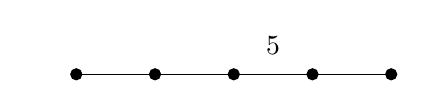
\begin{tikzpicture}[scale=1.0]
\draw[fill=black] \foreach \x in {1,2,...,5} {(\x,1.5) circle (2pt)};%\widetilde{F}_{4}
\draw {(.5,1.5) node{}
(3.5,1.5) node[label=above:$5$]{}
[-] (1,1.5) -- (5,1.5)
(2,1.5) node{}}; 
\end{tikzpicture}
\caption{$\widetilde{F}_{4}$} \label{fig:H}
\end{subfigure} &

\begin{subfigure}{0.5\textwidth} \centering
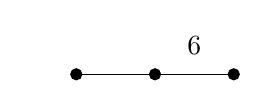
\begin{tikzpicture}[scale=1.0]
\draw[fill=black] \foreach \x in {1,2,...,3} {(\x,1.5) circle (2pt)};%\widetilde{G}_{2}
\draw {(.5,1.5) node{}
(2.5,1.5) node[label=above:$6$]{}
[-] (1,1.5) -- (3,1.5)
(2,1.5) node{}}; 
\end{tikzpicture}
\caption{$\widetilde{G}_{4}$} \label{fig:H}
\end{subfigure}
\end{tabular}
\caption{Coxeter graphs corresponding to the irreducible affine Coxeter groups}
\label{fig:infincoxgraphs}
\end{figure}

%%%%%%%%%%%%%%%%%%%%%%%%%%%


\section{Fully Commutative Elements}\label{sec:FC}
Let $(W,S)$ be a Coxeter system of type $\Gamma$ and let $w \in W$. Following~\cite{Stembridge1996}, we define a relation $\sim$ on the set of reduced expressions for $w$. Let $\overline{w}_1$ and $\overline{w}_2$ be two reduced expressions for $w$. We define $\overline{w}_1 \sim \overline{w}_2$ if we can obtain $\overline{w}_2$ from $\overline{w}_1$ by applying a single commutation move of the form $st \mapsto ts$ where $m(s,t)=2$. Now, define the equivalence relation $\approx$ by taking the reflexive transitive closure of $\sim$. Each equivalence class under $\approx$ is called a \emph{commutation class}. If $w$ has a single commutation class, then we say that $w$ is \emph{fully commutative} (FC). 

The set of FC elements of $W(\Gamma)$ is denoted by $\FC(\Gamma)$. We say that a reduced expression $\overline{w}$ is $\FC$ if it is a reduced expression for $w \in \FC(\Gamma)$. Given some $w \in \FC(\Gamma)$ and some starting expression for $w$, observe that the definition of FC states that to obtain all the reduced expressions for $w$, one only needs to perform commutations. The following theorem tells us that when $w$ is $\FC$, performing commutations is the only possible way to another reduced expression for $w$.

\begin{theorem}[Stembridge,~\cite{Stembridge1996}]
	An element $w \in W$ is FC if and only if no reduced expression for $w$ contains $\underbrace{sts\cdots}_{m(s,t)}$ as a subword for all when $m(s,t) \geq 3$. \qed
\end{theorem}

\begin{example}
	Let $w \in W(\widetilde{C}_4)$ and let $\overline{w}=s_0s_1s_2s_0s_3s_1$ be a reduced expression for $w$. We see that
	\[s_0s_1\textcolor{purple}{s_2s_0}s_3s_1=s_0s_1s_0s_2\textcolor{purple}{s_3s_1}=s_0s_1s_0s_2s_1s_3,\]
	where the \textcolor{purple}{purple} indicates applying a commutation. Note that there is no possible way to perform a braid move. Hence $w$ is $\FC$.
\end{example}

\begin{example}
Let $w \in W(\widetilde{C}_4)$ and let $\overline{w}=s_0s_1s_2s_0s_1s_2$ be a reduced expression for $w$. We see that
\[s_0s_1\textcolor{purple}{s_3s_0}s_1s_2=s_0s_1s_0\textcolor{purple}{s_3s_1}s_2=\textcolor{orange}{s_0s_1s_0s_1}s_3s_2,\]
where the \textcolor{purple}{purple} indicates applying a commutation and the \textcolor{orange}{orange} indicates applying a braid move. Thus $w$ is not $\FC$ since a braid move can be applied.  	
\end{example}

\begin{example}
Let $\overline{w}=s_1s_0s_4s_1s_3s_5s_2s_4s_6$ for $w \in \FC(\widetilde{C}_6)$. Applying the commutation $s_4s_2=s_2s_4$, we can obtain another reduced expression for $w$, namely $\overline{w}_2=s_1s_0s_4s_1s_3s_5s_4s_2s_6$ which is in the same commutation class as $\overline{w_1}$. However, applying the braid move $s_2s_3s_2=s_3s_2s_3$, we obtain another reduced expression $\overline{w_3}=s_1s_3s_2s_3s_4s_0$. Note that since $\overline{w}_3$ was obtained by applying a braid move, $\overline{w_3}$ is in a different commutation class than $\overline{w_1}$ and $\overline{w_2}$. It turns out $w$ has exactly two commutation classes, one containing $\overline{w}_1$ and $\overline{w}_2$ and another containing $\overline{w}_3$.
\end{example}


Stembridge classified the irreducible Coxeter groups that contain a finite number of fully commutative elements, the so-called \emph{FC-finite Coxeter groups}. This thesis is mainly concerned with $W(A_n),~W(B_n),~W(\widetilde{C}_n)$. Both $W(A_n),~W(B_n)$ are finite Coxeter groups, and thus are $\FC$-finite. On the other hand, $W(\widetilde{C}_n)$ is infinite and has infinitely many $\FC$ elements. However, there exist some infinite Coxeter groups that contain finitely many $\FC$ elements. For example, $E_n$ for $n \geq 9$ (see Figure~\ref{fig:infincoxgraphs}) is infinite, but contains only finitely many FC elements.

\begin{theorem}[Stembridge,~\cite{Stembridge1996}]
\label{thm:FCfinite} The FC-finite irreducible Coxeter groups are of type $A_n$ with $n \geq 1$, $B_n$ with $n \geq 2$, $D_n$ with $n \geq 4$, $E_n$ with $n \geq 6$, $F_n$ with $n \geq 4$, $H_n$ with $n \geq 3$, and $I_2(m)$ with $5 \leq m < \infty$. The corresponding Coxeter graphs are shown in Figures~\ref{fig:fincoxgraphs} and~\ref{fig:infincoxgraphs}. \qed
\end{theorem}
  


%%%%%%%%%%%%%%%%%%%%%%%%%%%


\section{Heaps}\label{sec:Heaps}

We can now discuss a visual representation of Coxeter group elements. Each reduced expression can be associated with a labeled partially ordered set (poset) called a heap.  Heaps provide a visual representation of a reduced expression while preserving the relations among the generators. We follow the development of heaps of straight line Coxeter groups in~\cite{Billey2007},~\cite{Ernst2010}, and~\cite{Stembridge1996}. 

Let $(W,S)$ be a Coxeter system of type $\Gamma$. Suppose $\overline{w}=s_{x_1}s_{x_2}\cdots s_{x_r}$ is a fixed reduced expression for $w \in W$. As in~\cite{Stembridge1996}, we define a partial ordering on the indices $\{1, 2, \ldots, r\}$ by the transitive closure of the relation $\lessdot$ defined via $j \lessdot i$ if $i < j$ and $s_{x_i}$ and $s_{x_j}$ do not commute. In particular, since $\overline{w}$ is reduced, $j \lessdot i$ if $s_{x_i}=s_{x_j}$ by transitivity. This partial order is referred to as the \emph{heap} of $\overline{w}$, where $i$ is labeled by $s_{x_i}$. Note that for simplicity we are omitting the labels of the underlying poset but retaining the labels of the corresponding generators.

It follows from~\cite{Stembridge1996} that heaps are well-defined up to commutation class. That is, given two reduced expressions $\overline{w}$ and $\overline{w'}$ for $w \in W$ that are in the same commutation class, then the heaps for $\overline{w}$ and $\overline{w'}$ will be equal. In particular, if $w \in \FC(\Gamma)$, then $w$ has a one commutation class, and thus $w$ has a unique heap.

When $w$ is $\FC$, we wish to make a canonical choice for the representation of $H(w)$ by assembling the entries in a particular way. To do so, we position all of the entries corresponding to elements in $\mathcal{L}(w)$ in the same vertical position, and all of the remaining elements should be positioned as high as possible in the lattice point representation. For example, the representation in Figure~\ref{fig:FC heap} is the canonical representation for $w$. Note that our canonical representation of heaps corresponds to Cartier-Foata normal form for monomials~\cite{Cartier1969, Green2006a}. \textcolor{red}{See Fox page 8 regarding a clever way to talk about non-fc heaps}. When illustrating heaps we will often stick to the canonical choice, and when illustrating the heaps of arbitrary reduced expressions we will discuss the relative position of the entries but never the absolute coordinates. 

\begin{example}
Let $\overline{w}=s_1s_0s_4s_1s_3s_5s_2s_4s_6$ be a reduced expression for $w \in \FC(\widetilde{C}_6).$ We see that $\overline{w}$ is indexed by $\{1,2,3,4,5,6,7,8,9\}$. As an example, $1 \lessdot 0$ since $0 <1$ and $s_0$ and $s_1$ do not commute. The labeled Hasse diagram for the heap poset is seen in Figure~\ref{fig:Hasse}.
\begin{figure}[h]
\centering
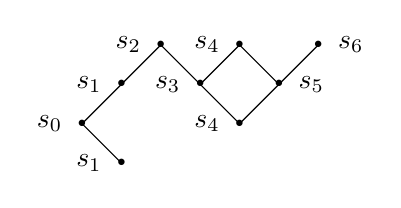
\begin{tikzpicture}[scale=0.5]
	\node[scale=0.6, label=left:$s_{2}$] at (2,5.5) {$\bullet$};
	\node[scale=0.6, label=left:$s_{4}$] at (4,5.5) {$\bullet$};
	\node[scale=0.6, label=right:$s_{6}$] at (6,5.5) {$\bullet$};
	\node[scale=0.6, label=left:$s_{1}$] at (1,4.5) {$\bullet$};
	\node[scale=0.6, label=left:$s_{3}$] at (3,4.5) {$\bullet$};
	\node[scale=0.6, label=right:$s_{5}$] at (5,4.5) {$\bullet$};
	\node[scale=0.6, label=left:$s_{0}$] at (0,3.5) {$\bullet$};
	\node[scale=0.6, label=left:$s_{4}$] at(4,3.5) {$\bullet$};
	\node[scale=0.6, label=left:$s_{1}$] at (1,2.5) {$\bullet$};
\draw (1,2.5)--(0,3.5)--(1,4.5)--(2,5.5)--(3,4.5)--(4,3.5);
\draw (3,4.5)--(4,5.5)--(5,4.5)--(4,3.5);
\draw (6,5.5)--(5,4.5);
\end{tikzpicture}
\caption{Labeled hasse diagram for the heap of an element in $\FC(\widetilde{C}_n)$}
\label{fig:Hasse}	
\end{figure}
\end{example}

Let $\overline{w}$ be a reduced expression for an element in $w \in W(\widetilde{C}_n)$. As in~\cite{Billey2007} and~\cite{Ernst2010} we can represent a heap for $\overline{w}$ as a set of lattice points embedded in $\{0,1,2,\ldots, n\} \times \mathbb{N}$. To do so, we assign coordinates (not unique) $(x,y) \in \{0,1,2,\ldots, n\} \times \mathbb{N}$ to each entry of the labeled Hasse diagram for the heap of $\overline{w}$ in such a way that:
\begin{enumerate}
\item An entry with coordinates $(x,y)$ is labeled $s_i$ (or $i$) in the heap if and only if $x = i$; 

\item If an entry with coordinates $(x,y)$ is greater than an entry with coordinates $(x',y')$ in the heap then $y > y'$.
\end{enumerate}

Although the above is specific to $W(\widetilde{C}_n)$, the same construction works for any straight line Coxeter graph with the appropriate adjustments made to the label set and assignments of coordinates. Specifically for type $A_n$ our label set is $\{1,2, \ldots, n\}~\times~\mathbb{N}$ and for type $B_n$ our label set is $\{0,1, \ldots, n-1\} \times \mathbb{N}$.

In the case of any straight line Coxeter graph it follows from the definition that $(x,y)$ covers $(x',y')$ in the heap if and only if $x = x' \pm 1$, $y > y'$, and there are no entries $(x'', y'')$ such that $x'' \in \{x, x'\}$ and $y'< y'' < y$. This implies that we can completely reconstruct the edges of the Hasse diagram and the corresponding heap poset from a lattice point representation. The lattice point representation can help us visualize arguments that are potentially complex. Note that in our heaps the entries in the top correspond to the generators occurring in the right descent set of the corresponding reduced expression.

Let $\overline{w}$ be a reduced expression for $w \in W(\widetilde{C}_n)$. We denote the lattice representation of the heap poset in $\{0,1,2, \ldots n\} \times n$ described in the preceding paragraphs via $H(\overline{w})$. If $w$ is $\FC$, then the choice of reduced expression for $w$ is irrelevant and we will often write $H(w)$ (note the absence of \textsf{sans serif} font) and we refer to $H(w)$ as the heap of $w$. As above the necessary adjustments to the lattice representation will result in a general result for heaps of all straight line coxeter graphs.

Given a heap, there are many possible coordinate assignments, yet the $x$-coordinates will be fixed for each entry will be fixed for all of them. In particular, two entries labeled by the same generator will only differ by the amount of vertical space between them while they will maintain the same horizontal position to adjacent entries in the heap.

Let $\overline{w}=s_{x_1}s_{x_2}\cdots s_{x_r}$ be a reduced expression for $w \in W(\widetilde{C}_n)$. If $s_{x_i}$ and $s_{x_j}$ are adjacent generators in the Coxeter graph with $i<j$, then we must place the point labeled by $s_{x_j}$ at a level that is \emph{above} the level of the point labeled by $s_{x_i}$. Because generators in a Coxeter graph that are not adjacent do commute, points whose $x$-coordinates differ more than one can slide past each other or land in the same level. To emphasize the covering relations of the lattice point representation we will enclose each entry in the heap in a square with rounded corners in such a way that if one entry covers another the squares overlap halfway. In addition, we will also label each square with $i$ representing the generator $s_i$.

\begin{example}
	Let $\overline{w}=s_1s_0s_4s_1s_3s_5s_2s_4s_6$ be a reduced expression for $w \in \FC(\widetilde{C}_6)$ as seen in Example 1.4.1. Figure~\ref{fig:FC heap} shows a possible lattice point representation for $H(w)$.
\begin{figure}[h]
\centering
\begin{tikzpicture}[scale=0.4]
\heapblock{2}{6}{2}{purple}
\heapblock{4}{6}{4}{purple}
\heapblock{6}{6}{6}{purple}
\heapblock{1}{4}{1}{purple}
\heapblock{3}{4}{3}{purple}
\heapblock{5}{4}{5}{purple}
\heapblock{0}{2}{0}{purple}
\heapblock{4}{2}{4}{purple}
\heapblock{1}{0}{1}{purple}
\end{tikzpicture}
\caption{A possible lattice point representation of for the heap of an FC element in $W(\widetilde{C}_6)$.}
\label{fig:FC heap}
\end{figure}
\end{example}

\begin{example}
Let $\overline{w}_1=s_1s_2s_3s_4s_2s_0$ be a reduced expression for $w \in W(\widetilde{C}_4)$. Applying the commutation $s_4s_2=s_2s_4$, we can obtain another reduced expression for $w$, namely $\overline{w}_2$ which is in the same commutation class as $\overline{w_1}$ and hence has the same heap. However, applying the braid move $s_2s_3s_2=s_3s_2s_3$, we obtain another reduced expression $\overline{w_3}=s_1s_3s_2s_3s_4s_0$. Note that since $\overline{w}_3$ was obtained by applying a braid move, $\overline{w_3}$ is in a different commutation class than $\overline{w_1}$ and $\overline{w_2}$. Representations of $H(\overline{w}_1), H(\overline{w}_2)$ and $H(\overline{w_3})$ are seen in Figure~\ref{fig:not FC} where the braid relation is colored in orange.

\begin{figure}[h]
\centering
\begin{subfigure}[b]{0.3\textwidth}	
\centering
\begin{tikzpicture}[scale=0.4]
\heapblock{0}{6}{0}{purple}
\heapblock{2}{6}{2}{orange}
\heapblock{4}{6}{4}{purple}	
\heapblock{3}{4}{3}{orange}
\heapblock{2}{2}{2}{orange}
\heapblock{1}{0}{1}{purple}
\end{tikzpicture}
\caption{$H(\overline{w}_1)$ and $H(\overline{w}_2)$ in $W(\widetilde{C}_4$.}
\end{subfigure}
\begin{subfigure}[b]{0.3\textwidth}	
\centering
\begin{tikzpicture}[scale=0.4]
\heapblock{10}{6}{0}{purple}
\heapblock{14}{6}{4}{purple}
\heapblock{13}{4}{3}{orange}
\heapblock{12}{2}{2}{orange}
\heapblock{11}{0}{1}{purple}
\heapblock{13}{0}{3}{orange}
\end{tikzpicture}
\caption{$H(\overline{w}_3)$}
\end{subfigure}
\caption{Two heaps of a non-FC element}	
\label{fig:not FC}
\end{figure}
\end{example}



%%%%%%%%%%%%%%%%%%%%%%%%%%%%%%%%%%

\section{Star Operations and Non-Cancellable Elements}\label{Star}

The notion of star operations was originally introduced by Kazhdan and Lusztig in~\cite{Kazhdan1979} for simply laced Coxeter systems (i.e., $m(s,t) \leq 3$ for all $s,t \in S$), and was later generalized to all Coxeter systems in~\cite{Lusztig1985}. If $I=\{s,t\}$ is a pair of non-commuting generators of a Coxeter group $W$, then $I$ induces four partially defined maps from $W$ to itself, known as \emph{star operations}. A star operation, when it is defined, increases or decreases the length of an element to which it is applied by 1. For our purposes it is enough to define only the star operations that decrease the length of an element by 1, and as a result we will not develop the notion in full generality.

\textcolor{red}{Dana will you make sure that this definition is correct.} Let $(W,S)$ be a Coxeter system of type $\Gamma$ and let $I=\{s,t\}\subseteq S$ be a pair of noncommuting generators whose product has order $m$. Let $w \in W(\Gamma)$ such that $s \in \mathcal{L}(w)$. We define $w$ to be \emph{left star reducible by $s$ with respect to $t$} if there exists $t \in \mathcal{L}(sw)$. We analogously define $w$ to be \emph{right star reducible by $s$ with respect to $t$}. Observe that if $m(s,t) \geq 3$, then $w$ is left (respectively, right) star reducible if and only if there is a reduced expression for $w$ such that $\overline{w}=stv$ (respectively, $\overline{w}=vts$). We say that $w$ is \emph{star reducible} if it is either left or right star reducible.

\begin{example}
Let $w \in W(B_4)$ and let $\overline{w}=s_0s_1s_0s_2s_3$ be a reduced expression for $w$. We see that $w$ is left star reducible by $s_0$ with respect to $s_1$ to $s_1s_0s_2s_3$, since $m(s_0,s_1)=4$ and $s_0 \in \mathcal{L}(w)$ while $s_1 \in \mathcal{L}(s_0w)$. Also $w$ is right star reducible by $s_3$ with respect to $s_2$ to $s_0s_1s_0s_2$, since $m(s_2,s_3)=3$ and $s_3 \in \mathcal{R}(w)$ and $s_2 \in \mathcal{R}(ws_3)$.
\end{example}
 
We now introduce the concept of weak star reducible which is related to the notion of cancellable in~\cite{Fan1997}. Let $(W,S)$ be a Coxeter system of type $\Gamma$ and let $I=\{s,t\} \subseteq S$ be a pair of noncommuting generators of the Coxeter group $W(\Gamma)$. If $w  \in \FC(\Gamma)$, then $w$ is \emph{left weak star reducible by $s$ with respect to $t$ to $sw$} if
\begin{enumerate}
\item $w$ is left star reducible by $s$ with respect to $t$;
\item and $tw \notin \FC(W)$.	
\end{enumerate}
Notice that (2) implies that $l(tw)>l(w)$. Also note that we are restricting out definition of weak star reducible to the set of $\FC$ elements of $W(\Gamma)$. We analogously define \emph{right weak star reducible by $s$ with respect to $t$ to $ws$}. We say that $w$ is \emph{weak star reducible} if $w$ is either left or right weak star reducible. Otherwise, we say that $w$ is \emph{non-cancellable} or \emph{weak star irreducible}.

\begin{example}
Let $w \in \FC(B_4)$ and let $\overline{w}=s_0s_1s_0s_2s_3$ be a reduced expression for $w$ as in Example 1.5.1. By Example 1.5.1 we know that $w$ is left star reducible. Also, $tw=s_1s_0s_1s_0s_2s_3$ which is not in $\FC(B_4)$. Thus, we see that $w$ is left weak star reducible by $s_0$ with respect to $s_1$ to $s_1s_0s_2s_3$. In addition, Example 1.5.1 showed that $w$ is right star reducible. Also, $wt=s_0s_1s_0s_2s_3s_2$ which is not in $\FC(B_4)$. Thus, we see that $w$ is right weak star reducible by $s_3$ with respect to $s_2$ to $s_0s_1s_0s_2$. This implies that $w$ is not non-cancellable.
\end{example}

\begin{example}
Let $w \in \FC(B_4)$ and let $\overline{w}=s_0s_1s_2$ be a reduced expression for $w$. Note that $w$ is left (respectively, right) star reducible by $s_0$ with respect to $s_1$ (respectively, by $s_2$ with respect to $s_1$). However, $s_1s_2 \in \FC(B_4)$ (respectively, $s_0s_1 \in \FC(B_4)$). Thus $w$ is non-cancellable.
\end{example}

Using the notion of star reducible we are now able to introduce the concept of a star reducible Coxeter group. We say that a Coxeter group $W(\Gamma)$, or it's Coxeter graph $\Gamma$, is \emph{star reducible} if every element of $\FC(\Gamma)$ is star reducible to a product of commuting generators. That is, $W(\Gamma)$ is star reducible if when we apply star operations repeatedly to $w \in \FC(\Gamma)$ and eventually $w$ is a product of commuting generators. In\cite{Green2006a}, Green classified all star reducible Coxeter groups. The Coxeter groups $W(A_n)$, $W(B_n)$ and $W(\widetilde{C}_n)$ are star reducible. However, $W(A_n)$ and $W(B_n)$ don't have non-trivial T-avoiding elements, while $W(\widetilde{C}_n)$ in one parity does have non-trivial T-avoiding elements.
\begin{theorem}
	Let $W(\Gamma)$ be a Coxeter group with (finite) generating set $S$. Then $W(\Gamma)$ is star reducible if an only if each component of $\Gamma$ is either a complete graph with labels $m(s,t)\geq 3$, or is one of the following types: type $A_n$ $(n \geq 1)$, type $B_n$ $(n \geq 2)$, type $D_n$ $(n \geq 4)$, type $F_n$ $(n \geq 4)$, type $H_n$ $(n \geq 2)$, type $I_2(m)$ $(m \geq 3)$, type $\widetilde{A}_{n-1}$ $(n \geq 3 \textrm{ and } n \textrm{ odd })$, type $\widetilde{C}_{n-1}$ $(n\geq 4 \textrm{ and } n \textrm{ even })$, type $\widetilde{E}_6$ or type $\widetilde{F}_5$. \qed
\end{theorem}  


%%%%%%%%%%%%%%%%%%%%%%%%%%%%%%%%
\section{Property T and T-Avoiding Elements}\label{Tavoid}

\textcolor{red}{Introduction and Motivation for this section}

We first begin by defining the notion of Property-T. Let $(W,S)$ be a Coxeter system of type $\Gamma$ and let $w \in W$ we say that $w$ has \emph{Property-T} if and only if there exists are reduced expression $\overline{w}$ such that $\overline{w}=stu$ or $\overline{w}=uts$ where $m(s,t)\geq 3$. That is, $w$ has Property-T if there exists a reduced expression for $w$ that begins with a product of non-commuting generators or ends with a product of non-commuting generators. It should be noted that by the symmetry of the definition if $w$ has Property-T, then $w^{-1}$ has Property-T

\begin{example}
Let $w \in W(A_5)$ and let $\overline{w}=s_1s_4s_2s_3s_5$. Note that applying a commutation to $s_4s_5$ results in $\overline{w}_1=s_1s_2s_4s_3s_5$. Hence $w$ has Property-T, since $m(s_1,s_2)=3$ and there is a reduced expression for $w$ which starts with $s_1s_2$.	
\end{example}

\begin{example}\label{ex:tavoid}
Let $w \in W(A_5)$ and let $\overline{w}=s_1s_3s_5$. It turns out that since $w$ is a product of commuting generators there is no reduced expression for $w$ that begins or ends with a pair of non-commuting generators. This implies that $w$ does not have Property-T.	
\end{example}

An element $w \in W(\Gamma)$ is called \emph{T-avoiding} if $w$ and $w^{-1}$ does not have Property-T. As seen in Example~\ref{ex:tavoid} an element $w \in W(\Gamma)$ will be T-avoiding if $w$ is a product of commuting generators. We will call an element that is a product of commuting generators \emph{trivially T-avoiding}. If $w$ is T-avoiding and not a product of commuting generators, we will say that $w$ is \emph{non-trivially T-avoiding.}

\begin{example}
Let $w \in W(A_5)$ and let $\overline{w}=s_1s_3s_5$. Then by Example~\ref{ex:tavoid}, we know that $w$ is T-avoiding. Furthermore, since $w$ is a product of commuting generators, $w$ is trivially T-avoiding.	
\end{example}

\begin{example}
Let $w \in W(\widetilde{C}_4)$ and let $\overline{w}=s_0s_2s_4s_1s_3s_0s_2s_4$. It turns out that $w$ is non-trivially T-avoiding. 	
\end{example}

